\section{Introduction}

\justifying
This chapter presents the analysis and specification of the \textbf{CyberScope} system. It introduces the adopted development methodology, identifies the main stakeholders, presents the development environment, and defines both functional and non-functional requirements. It also presents the use case diagram, the textual description of the main use cases, and the organization of the project through the product backlog and sprint planning.

\section{Adopted Development Methodology}

\justifying
To ensure a flexible and progressive development process, the Scrum methodology was adopted for the realization of \textbf{CyberScope}. Scrum is an agile framework based on iterative development, incremental delivery, continuous feedback, and adaptation to evolving requirements.

{\titlespacing*{\subsection}{1.0cm}{6pt}{3pt}
\subsection{Justification of the Choice of Scrum}
}

\justifying
The choice of Scrum is justified by the nature of the CyberScope project, which involves several heterogeneous components such as a frontend dashboard, a backend API, a Python-based scanning engine, external security tools, and AI-based analysis modules.

A traditional sequential development approach would make it difficult to validate each component progressively. Scrum allows the project to be divided into smaller increments, making it possible to test, validate, and improve each part of the system throughout development; this iterative approach is illustrated in Figure~\ref{fig:scrum-cyberscope}, which shows the sprint cycles, ceremonies, and feedback loops that guided the three project sprints.

\begin{figure}[H]
    \centering
    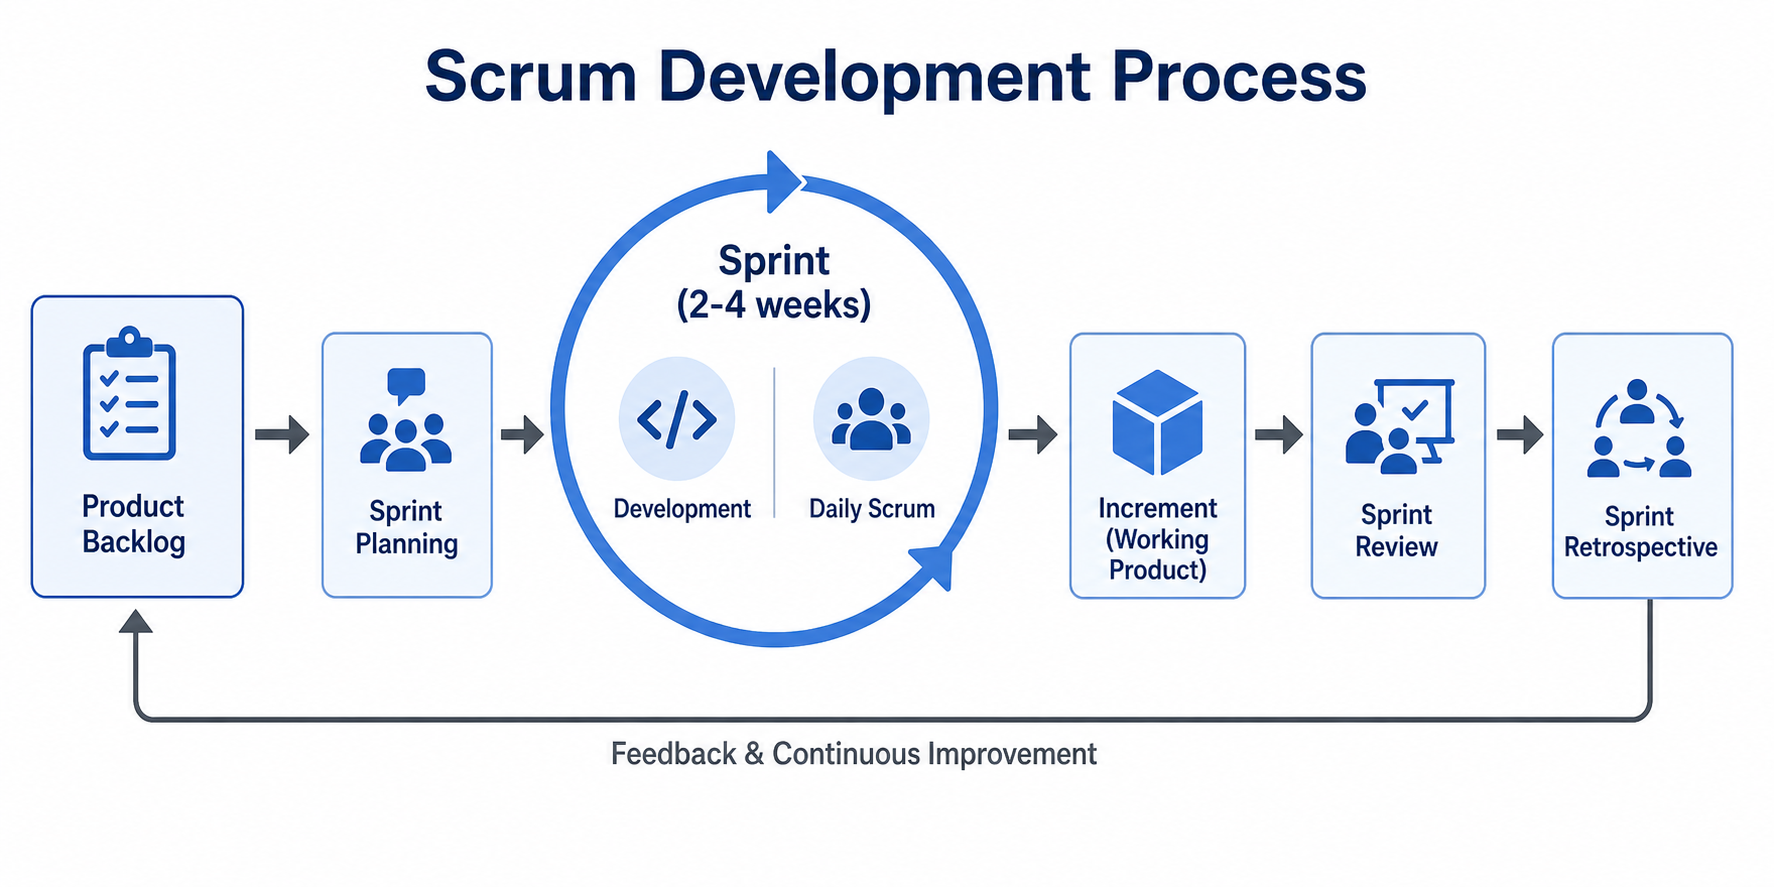
\includegraphics[width=1\textwidth]{uploads/images/scrum.png}
    \caption{Scrum Development Process adapted to CyberScope}
    \label{fig:scrum-cyberscope}
\end{figure}

\subsection{Organization of Sprints }

\vspace{0.4cm}

\indent CyberScope is organized into three iterative sprints, each with distinct objectives and deliverables; each sprint delivers a cohesive set of user stories aligned with its main objective. Table~\ref{tab:sprint-organization} presents the sprint timeline and main goals, showing progress from backend infrastructure through tool integration to attack graph generation over a 12-week development cycle.
\begin{table}[H]
    \centering
    \caption{Sprint Organization of CyberScope}
    \label{tab:sprint-organization}
    \renewcommand{\arraystretch}{1.25}
    \begin{tabularx}{\textwidth}{|p{1.8cm}|X|X|p{1.8cm}|}
        \hline
        \textbf{Sprint} & \textbf{Main Objective} & \textbf{Deliverable} & \textbf{Duration} \\
        \hline
        Sprint 1 & Backend foundation and database setup & Core backend APIs and database structure & 4 weeks \\
        \hline
        Sprint 2 & Scanning engine and tool orchestration & Integration of tools and scanning pipeline & 4 weeks \\
        \hline
        Sprint 3 & Attack Graph Generation & Computational framework for generating attack graphs & 4 weeks \\
        \hline
    \end{tabularx}
    \end{table}


\subsection{Backlog estimation methods}

User stories were estimated using a T‑shirt sizing approach (XS–XL) that favors relative effort over numeric points. This simplifies comparisons of complexity across backlog items; the adopted sizing scale is shown in Figure~\ref{fig:tshirt-sizing}.

\begin{figure}[H]
    \centering
    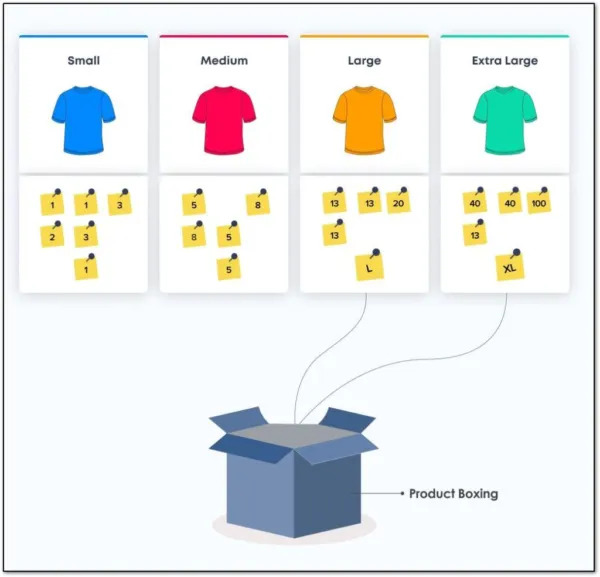
\includegraphics[width=0.6\textwidth]{uploads/images/tshirt (1).jpg}
    \caption{T-shirt sizing method (XS--XL) used for coarse estimates}
    \label{fig:tshirt-sizing}
\end{figure}
 
\subsection{Product Backlog}

\indent\justifying The product backlog consolidates all identified user stories, features, and technical tasks prioritized for implementation. Table~\ref{tab:product-backlog} lists the backlog items with their assigned sprint, category, and priority, providing a roadmap for development and release planning.


    {\small
    \begin{longtable}{|>{\centering\arraybackslash}p{1.4cm}|>{\centering\arraybackslash}p{2cm}|>{\centering\arraybackslash}p{2.2cm}|>{\raggedright\arraybackslash}p{7.5cm}|>{\centering\arraybackslash}p{1.2cm}|}
        \caption{Product Backlog of CyberScope}
        \label{tab:product-backlog} \\
        \hline
        \textbf{ID} & \textbf{Sprint} & \textbf{Category} & \textbf{User Story} & \textbf{Priority} \\
        \hline
        \endfirsthead
        \multicolumn{5}{c}{\textit{}} \\
        \hline
        \textbf{ID} & \textbf{Sprint} & \textbf{Category} & \textbf{User Story} & \textbf{Priority} \\
        \hline
        \endhead
        \hline
        \multicolumn{5}{r}{\textit{continued on next page}} \\
        \endfoot
        \hline
        \endlastfoot
        US-S1-01 & Sprint 1 & Authentication & As a User, I can create an account and log in to the platform so that I can securely access my data and scanning features. & High \\
        \hline
        US-S1-02 & Sprint 1 & Session & As a Guest User, I can start a temporary guest session without creating a persistent account so that I can quickly evaluate the platform. & Medium \\
        \hline
        US-S1-03 & Sprint 1 & Access Control & As a User, I can access protected pages such as the scanner and scan history so that I can run scans and review past results. & High \\
        \hline
        US-S1-04 & Sprint 1 & Session Management & As the System, I can verify and refresh the current session by exposing the authenticated user profile so that sessions remain valid and secure. & High \\
        \hline
        US-S1-05 & Sprint 1 & Tool Integration & As the System, I must resolve and safely execute HexStrike scanner binaries with timeout enforcement and resource limits so that tool outputs are captured reliably for processing. & High \\
        \hline
        US-S1-06 & Sprint 1 & AI Foundation & As the System, I must integrate Ollama for local AI inference to enable contextual analysis and intelligent recommendation generation without external API dependencies. & High \\
        \hline
        US-S2-01 & Sprint 2 & Scan Submission & As a User, I can submit a scan target (URL) and receive a job identifier so that I can track and retrieve results. & High \\
        \hline
        US-S2-03 & Sprint 2 & Execution & As the System, I can run scanner tools and collect raw outputs so that findings can be processed. & High \\
        \hline
        US-S2-04 & Sprint 2 & Normalization & As the System, I can normalize raw outputs into a unified schema so that results are consistent across tools. & High \\
        \hline
        US-S2-05 & Sprint 2 & Matching & As the System, I can match normalized findings to the vulnerability catalog and assign severities so that results are actionable. & High \\
        \hline
        US-S2-06 & Sprint 2 & Results UI & As a User, I can view, filter, and export scan history and results so that I can analyze and share findings. & Medium \\
        \hline
        US-S2-07 & Sprint 2 & Operations & As the System, I can monitor queue status and worker health so that the processing pipeline remains reliable. & Medium \\
        \hline
        US-S3-01 & Sprint 3 & Scenario Gen & As a User, I can request an attack scenario for a specific vulnerability and receive structured steps and a graph object so that I can investigate exploitation paths. & High \\
        \hline
        US-S3-02 & Sprint 3 & Remediation & As a User, I can click on an attack scenario step in the interactive graph so that I receive contextualized remediation tips and countermeasures to address that specific vulnerability. & High \\
        \hline
        US-S3-03 & Sprint 3 & Normalization & As the System, I must validate and normalize AI responses into a safe, consistent graph payload (nodes/edges) so that frontend rendering is robust and secure. & High \\
        \hline
        US-S3-04 & Sprint 3 & Frontend Integration & As a User, the Dashboard should render the returned graph (React Flow) and allow interaction with attack scenario steps so that I can explore potential attack paths. & Medium \\
        \hline
        US-S3-05 & Sprint 3 & Operations & As the System, I should handle AI timeouts, malformed responses, and return useful error messages so that failures are observable and debuggable. & Medium \\
        \hline
    \end{longtable}
    }
% duplicate/older Product Backlog table removed (kept the sprint-assigned detailed backlog above)



\section{Stakeholder Identification}

\indent The development and use of \textbf{CyberScope} involve three primary actors, each interacting with the system according to specific roles and responsibilities.

\indent The \textbf{User} represents the primary actor and main beneficiary of the platform. This actor performs core activities such as creating an account, logging in, submitting target URLs for security analysis, launching scans, and analyzing results through the interactive dashboard. The User relies on the system to provide accurate vulnerability detection and actionable remediation recommendations.

\indent The \textbf{Guest User} is a secondary actor who interacts with the platform without establishing a persistent account. This actor can access the system through a temporary guest session to evaluate the platform's capabilities and explore basic features, enabling quick evaluation without registration overhead.

\indent The \textbf{System} acts as the backend orchestrator and automated processor.This actor performs critical operations including tool integration and resolution, session management, scan execution and pipeline orchestration, output normalization and enrichment, vulnerability matching, and AI-driven attack graph generation.The System ensures reliable, scalable, and secure operation of all automated processes.
\break
\section{System Overview}

\indent\justifying CyberScope is an intelligent web application security auditing platform designed to automate vulnerability detection and analysis. It integrates multiple security tools into a unified pipeline and provides advanced features such as dynamic crawling, result aggregation, and AI-driven interpretation.

\indent The system is composed of three main components:

\begin{itemize}
    \item A frontend dashboard for user interaction and visualization
    \item A backend orchestration layer managing scans and data
    \item A scanning engine responsible for executing security tools
\end{itemize}

\section{Functional Requirements}

\indent\justifying The functional requirements define the core services provided by CyberScope. These functionalities describe how the system interacts with users and how it performs automated security analysis, from scan initiation to result reporting.

\subsection{Scan Initiation and Target Submission}

\indent The system must allow users to submit a target web application through a valid URL and initiate a security scan. Prior to execution, the system must validate the input to ensure correctness and accessibility of the target.

\indent Once validated, the system must create a scan instance, assign it a unique identifier, and trigger the scanning workflow. The user must be able to monitor the progress of the scan (e.g., pending, running, completed, failed) through the interface. Additionally, the system should support multiple concurrent scans and maintain a history of previous scans for later consultation.

\subsection{Intelligent Tool Orchestration}

\indent CyberScope must coordinate the execution of multiple security tools within a unified and automated pipeline. The system should dynamically orchestrate tools such as Nmap, Nuclei, Nikto, and SQLMap depending on the target characteristics.

\indent The orchestration process must ensure efficient scheduling, avoid redundant executions, and support parallel processing when possible. It must also manage tool configuration, execution, and result collection transparently, without requiring manual user intervention.

\subsection{Dynamic Application Crawling (BrowserAgent)}

\indent The system must include a browser-based crawling component, referred to as the \textbf{BrowserAgent}, capable of interacting with modern web applications.

\indent This component must simulate real user behavior by executing JavaScript, navigating through dynamic interfaces, and capturing network requests. It enables the discovery of hidden endpoints, API calls, and parameters that are not accessible through traditional static scanning techniques.

\indent This functionality is particularly important for analyzing Single Page Applications (SPAs) and dynamically generated content.

\subsection{Vulnerability Detection and Analysis}

\indent The system must detect a wide range of web application vulnerabilities, including SQL injection, cross-site scripting (XSS), exposed services, insecure configurations, and outdated components.

\indent CyberScope must process the outputs of integrated tools and transform them into structured vulnerability objects. Each vulnerability should include detailed information such as its type, severity level, affected endpoint, technical evidence, and potential impact.

\indent This structured representation facilitates further analysis, prioritization, and decision-making.

\subsection{Aggregation and Visualization of Results}

\indent The system must aggregate results collected from multiple tools and eliminate duplicate findings through normalization and deduplication mechanisms.

\indent The processed results must be presented through an intuitive dashboard that allows users to explore vulnerabilities using filters, sorting options, and visual indicators. The interface should provide a clear overview of the security posture, including severity distribution, affected components, and scan statistics.

\indent This improves readability and enables users to quickly identify and prioritize critical issues.

\subsection{Report Generation}

\indent The system must generate comprehensive and structured reports summarizing the results of a security scan.

\indent These reports should include target information, detected vulnerabilities, severity classification, risk assessment, and remediation recommendations. The reports must be exportable in a professional format (e.g., PDF) to facilitate communication with stakeholders and support auditing processes.

\section{Non-Functional Requirements}

\indent Non-functional requirements define the quality attributes and operational constraints of the CyberScope system. They ensure that the platform is efficient, secure, reliable, and maintainable.

\subsection{Performance and Scalability}

\indent The system must provide acceptable performance in terms of response time and processing efficiency. While vulnerability scans may be resource-intensive, user interactions with the platform must remain responsive.

\indent The architecture should support scalability by allowing the distribution of system components (frontend, backend, scanning engine) to handle increasing workloads and larger target applications without significant performance degradation.

\subsection{Security Requirements}

\indent CyberScope must implement strong security mechanisms to protect user data and scan results. Authentication and authorization must be enforced using secure approaches such as JSON Web Tokens (JWT).

\indent Sensitive data must be protected against unauthorized access, and secure communication must be ensured between system components. Given the nature of the platform, maintaining confidentiality and integrity is essential.

\subsection{Usability}

\indent The platform must provide an intuitive and user-friendly interface that simplifies interaction with complex security data.

\indent The dashboard should present information in a clear and structured manner, allowing users to easily navigate between scans, analyze vulnerabilities, and access reports. Important elements such as severity levels and risk indicators should be highlighted to improve decision-making.

\subsection{Reliability and Availability}

\indent The system must ensure stable and reliable operation during scan execution and data processing. It should handle failures gracefully, such as tool crashes or network interruptions, without compromising data integrity.

\indent Appropriate logging and error-handling mechanisms must be implemented to support monitoring and debugging. The system should also maintain high availability with minimal downtime.

\subsection{Maintainability and Extensibility}

\indent CyberScope must be designed using a modular architecture that facilitates maintenance and future evolution.

\indent The system should allow easy integration of new security tools, updates to existing components, and modifications without affecting the overall system stability. Clear separation between components (frontend, backend, scanning engine) enhances maintainability.

\indent Extensibility is essential to adapt the platform to new vulnerabilities, technologies, and evolving security requirements.

\section{Global Use Case Diagram}

\indent The use case diagram illustrates the main interactions between the user and the CyberScope system; Figure~\ref{fig:global-usecase} shows the main actors (User, Guest User, and System) and the primary use case flows for authentication, scanning, and attack scenario generation.

\begin{figure}[H]
    \centering
    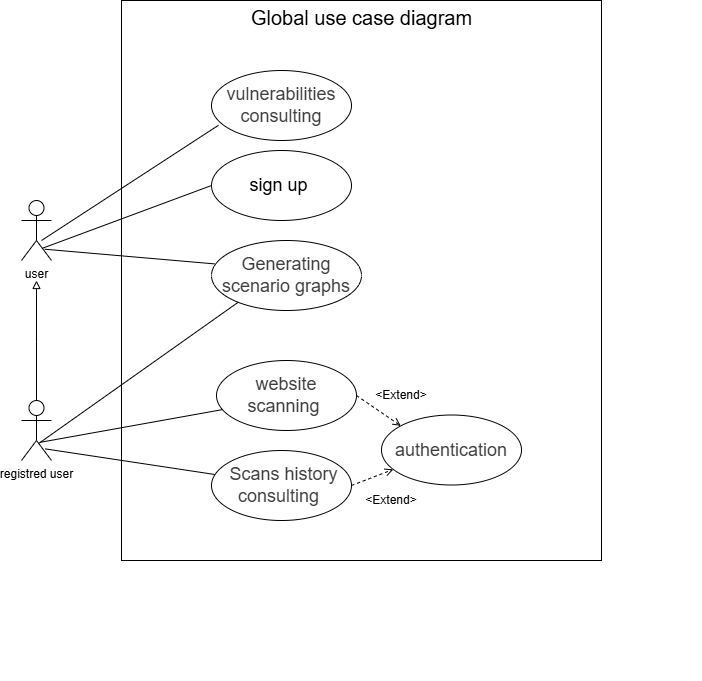
\includegraphics[width=0.85\textwidth]{uploads/diagrams/use case general .drawio.png}
    \caption{Global Use Case Diagram of CyberScope}
    \label{fig:global-usecase}
\end{figure}


\clearpage
\section{Global Class Diagram}


\vspace{0.3cm}

\indent The class diagram presents the main structural components of CyberScope and the relationships between its core services, models, and orchestration layers.
\noindent Figure~\ref{fig:global-class-diagram} presents the principal components and relationships of CyberScope architecture, including frontend models, backend API services, scanning engine, and external tool integration layers.

\begin{figure}[H]
    \centering
    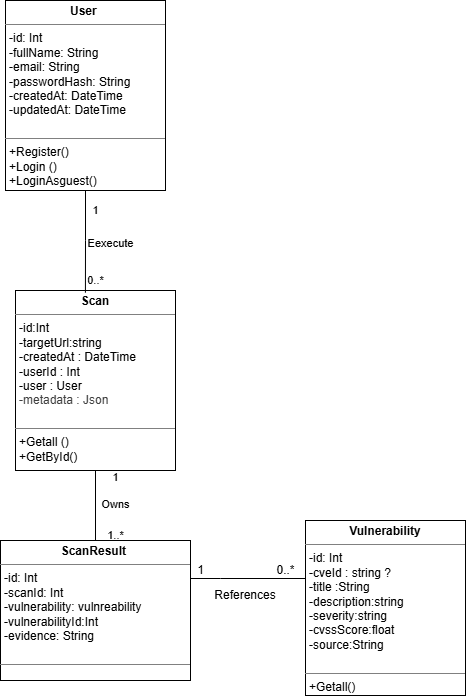
\includegraphics[width=0.8\textwidth]{uploads/diagrams/classglobal.drawio.png}
    \caption{Global Class Diagram of CyberScope}
    \label{fig:global-class-diagram}
\end{figure}

\section{Development Environment}

\indent This section presents the technical environment used to design, implement, and test \textbf{CyberScope}. It highlights the main programming languages, frameworks, tools, and software resources that supported the project.

\subsection{Material Environment}

\indent Development work was performed on a Windows workstation using the following primary tools; Figure~\ref{fig:vscode-logo} shows Visual Studio Code, the primary development environment used for writing frontend and backend code, providing advanced features for debugging and extension management.


\vspace{0.3cm}

\begin{figure}[H]
    \centering
    
\includegraphics[width=2.4cm]{uploads/logos/vscode.png}
    \caption{Logo of Visual Studio Code.}
    \label{fig:vscode-logo}
    \vspace{0.2cm}
    \begin{minipage}{0.9\textwidth}
        \centering
    \end{minipage}
\end{figure}
\indent Figure~\ref{fig:git-logo} represents Git, the distributed version control system used for managing source code, tracking development history, and coordinating collaborative contributions throughout the project lifecycle.

\vspace{0.3cm}
\begin{figure}[H]
    \centering
    
\includegraphics[width=2.4cm]{uploads/logos/git.png}
    \caption{Logo of Git.}
    \label{fig:git-logo}
    \vspace{0.2cm}
    \begin{minipage}{0.9\textwidth}
        \centering
    \end{minipage}
\end{figure}

\indent Figure~\ref{fig:chromium-logo} shows the Chromium/Google Chrome browser, used for manual functional testing, dynamic content verification, and network analysis of the CyberScope frontend during development.

\vspace{0.3cm}
\begin{figure}[H]
    \centering
    
\includegraphics[width=2.4cm]{uploads/logos/Chromium_Logo.png}
    \caption{Logo of Google Chrome / Chromium.}
    \label{fig:chromium-logo}
    \vspace{0.2cm}
    \begin{minipage}{0.9\textwidth}
        \centering
    \end{minipage}
\end{figure}

\indent Figure~\ref{fig:drawio-logo} represents diagrams.net (draw.io), the diagramming tool used to create all architectural diagrams, use case diagrams, class diagrams, and sequence diagrams throughout the documentation.

\vspace{0.3cm}
\begin{figure}[H]

    \centering
    
\includegraphics[width=2.4cm]{uploads/images/drawiologo.png}
    \caption{Logo of diagrams.net (draw.io).}
    \label{fig:drawio-logo}
    \vspace{0.2cm}
    \begin{minipage}{0.9\textwidth}
        \centering
    \end{minipage}
\end{figure}

\indent Figure~\ref{fig:overleaf-logo} shows Overleaf, the online collaborative LaTeX editor used for writing, editing, and compiling the project documentation and technical report.

\vspace{0.3cm}
\begin{figure}[H]
    \centering
    
\includegraphics[width=2.4cm]{uploads/images/overleaf-logo-primary.png}
    \caption{Logo of Overleaf.}
    \label{fig:overleaf-logo}
    \vspace{0.2cm}
    \begin{minipage}{0.9\textwidth}
        \centering
    \end{minipage}
\end{figure}


\subsection{Software Environment}

\indent The software stack is organized by layer; the following items present the main technologies with a short description for each.

\vspace{0.3cm}
\noindent\textbullet\ \textbf{Backend}

\vspace{0.2cm}

\indent Figure~\ref{fig:node-logo} represents Node.js, the JavaScript runtime environment providing the execution platform for the CyberScope backend server and all related processes.

\vspace{0.3cm}

\begin{figure}[H]
    \centering
    
\includegraphics[width=2.2cm]{uploads/logos/node.png}
    \caption{Node.js}
    \label{fig:node-logo}
    \vspace{0.2cm}
    \begin{minipage}{0.9\textwidth}
        \centering
    \end{minipage}
\end{figure}

\vspace{0.3cm}

\indent Figure~\ref{fig:express-logo} shows Express.js, the lightweight web framework used to define all RESTful API endpoints, routing logic, and middleware components in the CyberScope backend.

\vspace{0.3cm}

\begin{figure}[H]
    \centering
    
\includegraphics[width=2.2cm]{uploads/logos/Expressjs.png}
    \caption{Express.js}
    \label{fig:express-logo}
    \vspace{0.2cm}
    \begin{minipage}{0.9\textwidth}
        \centering
    \end{minipage}
\end{figure}

\vspace{0.3cm}


\vspace{0.3cm}
\indent Figure~\ref{fig:prisma-logo} shows Prisma, the Object-Relational Mapping tool providing type-safe database access, migrations, and schema management for the PostgreSQL database.

\begin{figure}[H]
    \centering
    
\includegraphics[width=2.2cm]{uploads/logos/prisma.jpg}
    \caption{Prisma}
    \label{fig:prisma-logo}
    \vspace{0.2cm}
    \begin{minipage}{0.9\textwidth}
        \centering
    \end{minipage}
\end{figure}

\vspace{0.3cm}

\indent Figure~\ref{fig:postgresql-logo} shows PostgreSQL, the robust relational database management system used to persistently store user data, scan jobs, vulnerabilities, and analysis results.

\vspace{0.3cm}

\begin{figure}[H]
    \centering
    
\includegraphics[width=2.2cm]{uploads/logos/postgresql.png}
    \caption{PostgreSQL}
    \label{fig:postgresql-logo}
    \vspace{0.2cm}
    \begin{minipage}{0.9\textwidth}
        \centering
    \end{minipage}
\end{figure}

\vspace{0.4cm}
\noindent\textbullet\ \textbf{Frontend} \\
\vspace{0.15cm}

\indent Figure~\ref{fig:react-logo} represents React, the JavaScript library used to build the interactive CyberScope frontend dashboard with reusable components, state management, and dynamic user interfaces.

\vspace{0.2cm}
\begin{figure}[H]
    \centering
    
\includegraphics[width=2.2cm]{uploads/logos/react.png}
    \caption{React}
    \label{fig:react-logo}
    \vspace{0.2cm}
    \begin{minipage}{0.9\textwidth}
        \centering
    \end{minipage}
\end{figure}


\vspace{0.3cm}

\indent Figure~\ref{fig:vite-logo} shows Vite, the modern frontend build tool and development server used to provide fast hot module replacement and optimized production builds for the React frontend.

\vspace{0.3cm}

\begin{figure}[H]
    \centering
    
\includegraphics[width=2.2cm]{uploads/logos/vite.jpg}
    \caption{Vite}
    \label{fig:vite-logo}
    \vspace{0.2cm}
    \begin{minipage}{0.9\textwidth}
        \centering
    \end{minipage}
\end{figure}

\vspace{0.3cm}

\indent Figure~\ref{fig:typescript-logo} represents TypeScript, the typed superset of JavaScript used throughout both frontend and backend development to provide static type checking and improved code quality.

\vspace{0.3cm}

\begin{figure}[H]
    \centering
    
\includegraphics[width=2.2cm]{uploads/logos/TS.png}
    \caption{TypeScript}
    \label{fig:typescript-logo}
    \vspace{0.2cm}
    \begin{minipage}{0.9\textwidth}
        \centering
    \end{minipage}
\end{figure}

\vspace{0.4cm}
\noindent\textbullet\ \textbf{Scanning \& AI Tools}

\indent Figure~\ref{fig:ollama-logo} shows Ollama, the local AI engine used to assist in analysis and prompt generation within CyberScope.

\vspace{0.3cm}
\begin{figure}[H]
    \centering
    
\includegraphics[width=2.2cm]{uploads/logos/ollama.png}
    \caption{Ollama}
    \label{fig:ollama-logo}
    \vspace{0.2cm}
    \begin{minipage}{0.9\textwidth}
        \centering
    \end{minipage}
\end{figure}
\indent Figure~\ref{fig:hexstrike-logo} shows HexStrike AI, the orchestration layer for automated execution of multiple security tools in CyberScope.

\vspace{0.3cm}
\begin{figure}[H]
    \centering
    
\includegraphics[width=2.2cm]{uploads/logos/hexstrike.png}
    \caption{HexStrike AI}
    \label{fig:hexstrike-logo}
    \vspace{0.2cm}
    \begin{minipage}{0.9\textwidth}
        \centering
    \end{minipage}
\end{figure}

% Diagramming and documentation tools are declared in Material Environment (2.8.1)



\section{Conclusion}

\indent This chapter presented the analysis and specification of the CyberScope system, including the adopted methodology, stakeholder identification, development environment, system overview, and requirements. These elements provide a solid foundation for the system design presented in the next chapter.
